\chapter{Introduction}
\label{chap:introduction}

\section{Background}

In the rapidly evolving landscape of speech processing technologies, the \textbf{Speech Gateway API} serves as a critical infrastructure for delivering advanced speech services to various applications. The Speech Gateway is a backend service that provides Speech-to-Text (STT) capabilities to end users through a secured API. It acts as a middle layer between client applications and an underlying Speech Engine, centralising authentication, access control, token issuance, and subscription management.

As the demand for speech processing services grows, the need for a robust, centralised management system becomes paramount. Traditionally, interacting with such APIs required direct integration and manual management, which can be inefficient for both end-users and administrators. The \textbf{Gateway Dashboard} project was initiated to bridge this gap, providing a user-friendly graphical interface that empowers users to manage their speech processing tasks while giving administrators the tools needed to oversee system operations and monetise services effectively.

\section{Problem Statement}

Prior to this project, the Speech Gateway ecosystem faced two main challenges. First, the existing system had \textbf{limited access control}, supporting only basic credentials without modern Single Sign-On (SSO) capabilities. Users had to create separate accounts and manage passwords manually, leading to credential fatigue and potential security risks from weak or reused passwords. Second, there was a complete \textbf{absence of monetisation infrastructure}---no automated system existed to handle subscriptions, billing, or tiered access plans, which hindered the commercial viability of the services.

\section{Project Objectives}

The primary objective of this project is to design and implement a comprehensive Gateway Dashboard and enhance the backend infrastructure to support commercial-grade features. The specific objectives are:

\begin{itemize}
    \item \textbf{SSO Integration:} Implement secure Single Sign-On with Google and Apple to streamline user authentication, reduce credential fatigue, and centralise identity management across services.

    \item \textbf{Payment Portal:} Design a subscription and payment module integrating Stripe to handle recurring billing, automated invoicing, and subscription lifecycle management.

    \item \textbf{Frontend Development:} Develop a web-based dashboard using Vue.js and Vuetify to provide an intuitive interface for users to access speech services and manage their accounts.
\end{itemize}

\section{Project Scope}

The project encompasses three major components that together form a complete platform for managing the Speech Gateway services.

The \textbf{SSO Authentication} component enables users to authenticate using their existing Google or Apple accounts, in addition to traditional email and password credentials. This includes secure token management with automatic refresh mechanisms, token blacklisting via Redis for immediate revocation, and session security measures to prevent unauthorised access.

The \textbf{Payment Portal with Stripe Integration} component handles monetisation through the Stripe payment platform, enabling tiered subscription plans with usage-based quotas. It includes hosted checkout sessions, webhook-based event processing for payment lifecycle events, versioned plan management with an admin interface, and real-time synchronisation between Stripe and the internal database.

The \textbf{Frontend Dashboard} component provides a complete Single Page Application (SPA) built with Vue.js and Vuetify. It features authentication pages with SSO integration, protected routing with role-based access control, subscription management with usage monitoring, and an admin interface for managing plans and users.

\section{Proposed System Overview}

This section presents the three main components of the proposed system, illustrating how each addresses the challenges identified in the problem statement.

\subsection{Single Sign-On (SSO) Authentication}

\textbf{Before:} Users needed to create separate credentials for the Speech Gateway, leading to credential fatigue and security risks from weak or reused passwords.

\textbf{After:} Users can now sign in with their existing Google or Apple accounts in a streamlined flow. The user clicks on an SSO button, the system redirects to the identity provider for authentication, and upon success, the user is automatically logged in and redirected to the dashboard. For first-time SSO users, a brief account completion step collects any additional required information before granting full access.

\begin{figure}[H]
    \centering
    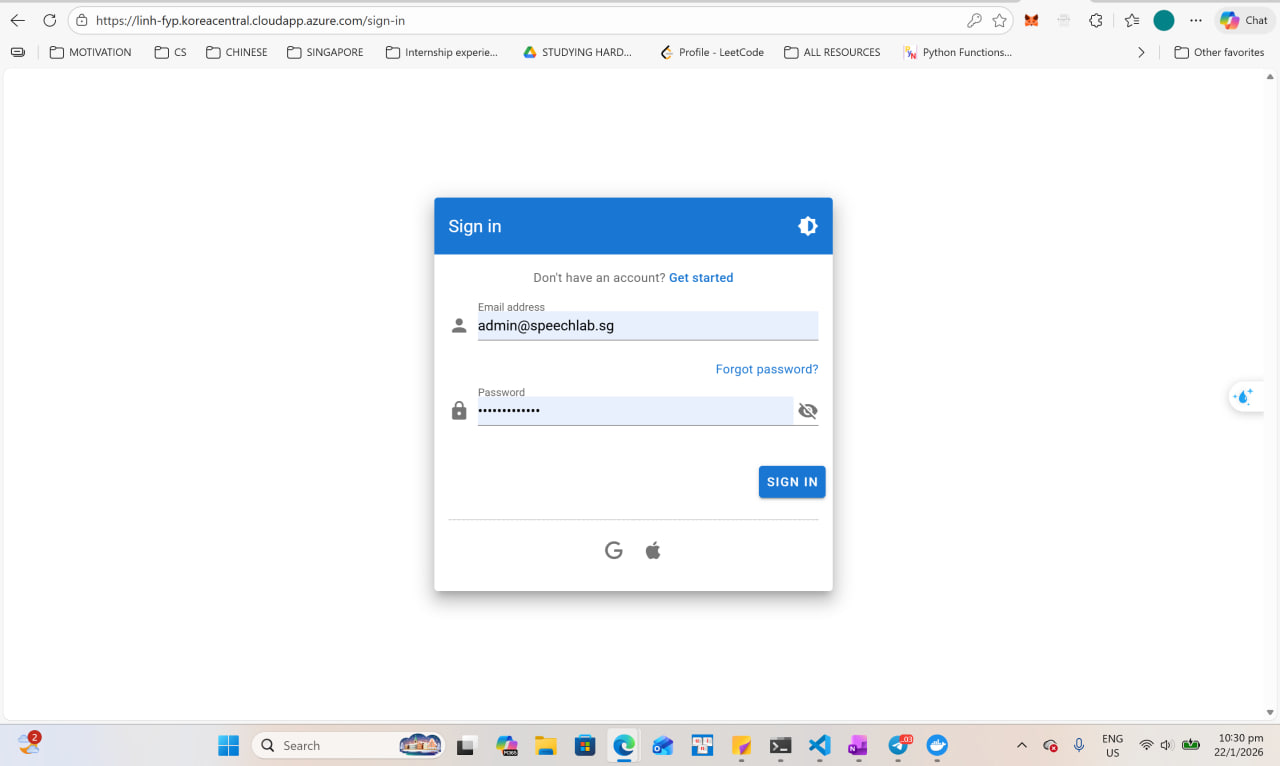
\includegraphics[width=0.8\textwidth]{images/Deployment/sign-in-UI.jpg}
    \caption{Sign-In Interface with SSO Options}
    \label{fig:sso-signin}
\end{figure}

\begin{figure}[H]
    \centering
    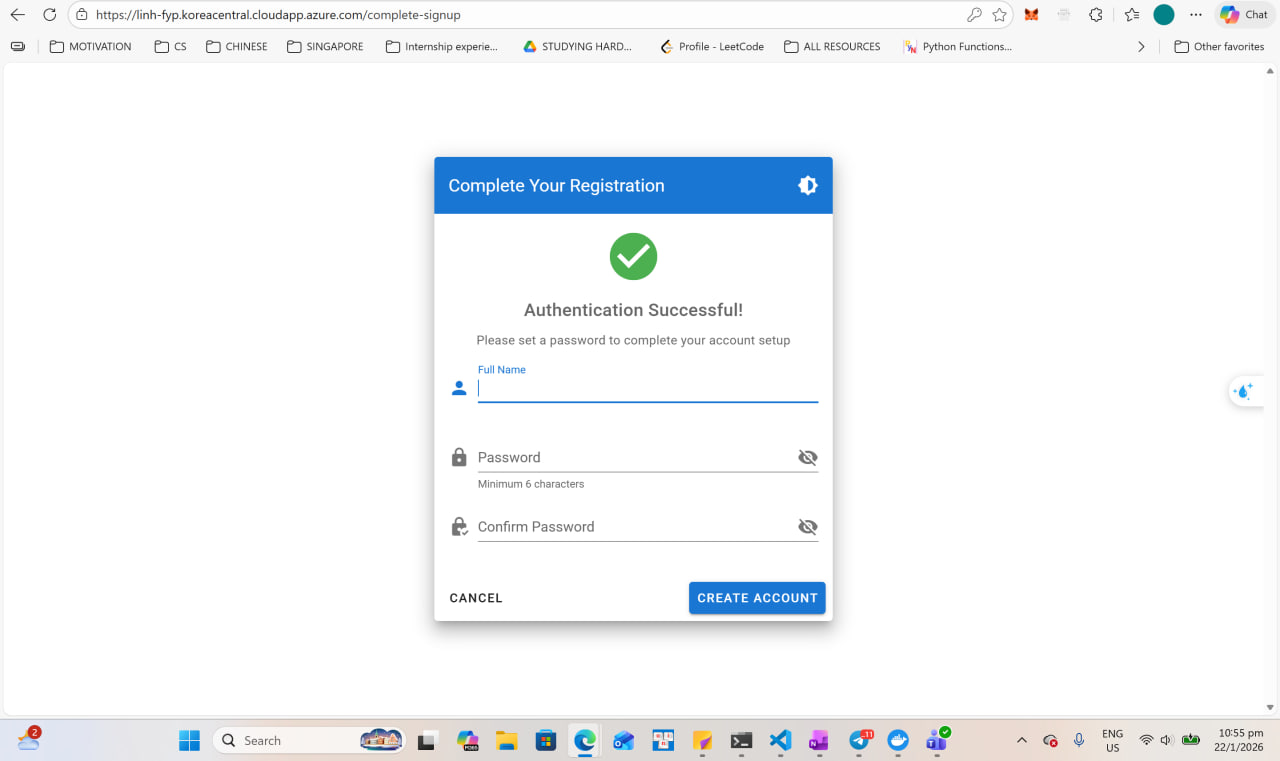
\includegraphics[width=0.8\textwidth]{images/Deployment/registration-UI.jpg}
    \caption{Registration Interface with SSO Integration}
    \label{fig:sso-registration}
\end{figure}

\subsection{Stripe Payment Integration}

\textbf{Before:} No automated billing existed, requiring manual invoice generation and payment verification before granting access to speech services.

\textbf{After:} The system now supports a fully automated payment flow. Administrators configure subscription plans in the Stripe product catalogue. When a user selects a plan and subscribes, the system creates a secure checkout session through Stripe's hosted page. Upon successful payment, Stripe notifies the system via webhooks, and the user's subscription status is automatically updated with the appropriate service quotas.

\begin{figure}[H]
    \centering
    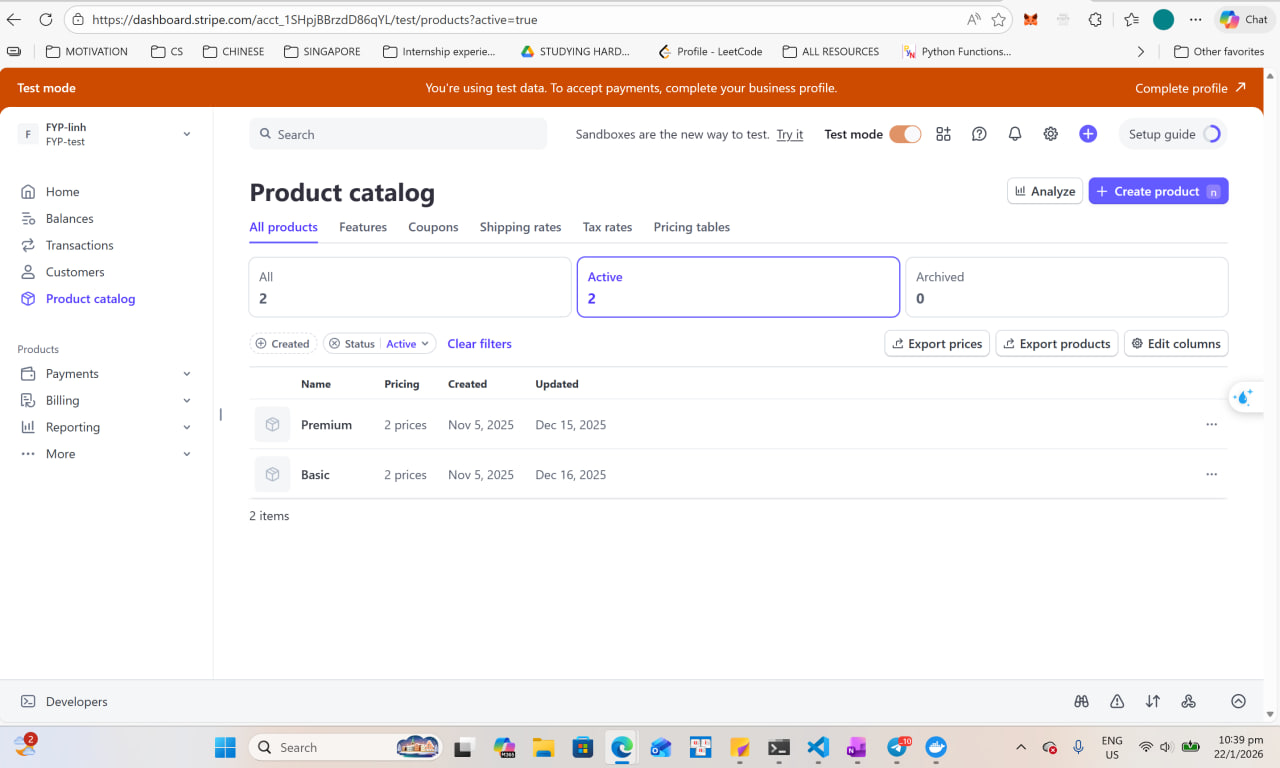
\includegraphics[width=0.8\textwidth]{images/Deployment/Stripe-product-catalog.jpg}
    \caption{Stripe Product Catalogue Configuration}
    \label{fig:stripe-catalog}
\end{figure}

\begin{figure}[H]
    \centering
    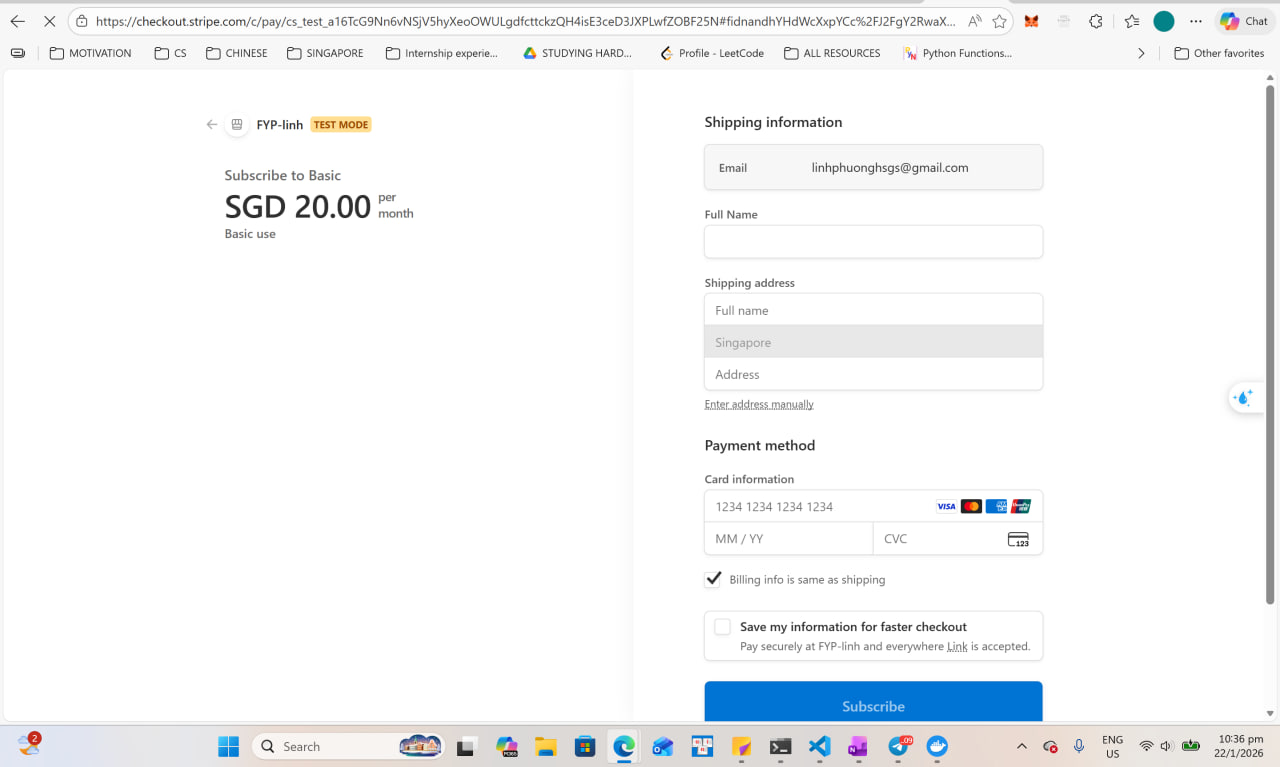
\includegraphics[width=0.8\textwidth]{images/Deployment/basic-plan-Stripe-check-out-UI-for-users.jpg}
    \caption{Stripe Checkout Interface for Basic Plan}
    \label{fig:stripe-checkout}
\end{figure}

\begin{figure}[H]
    \centering
    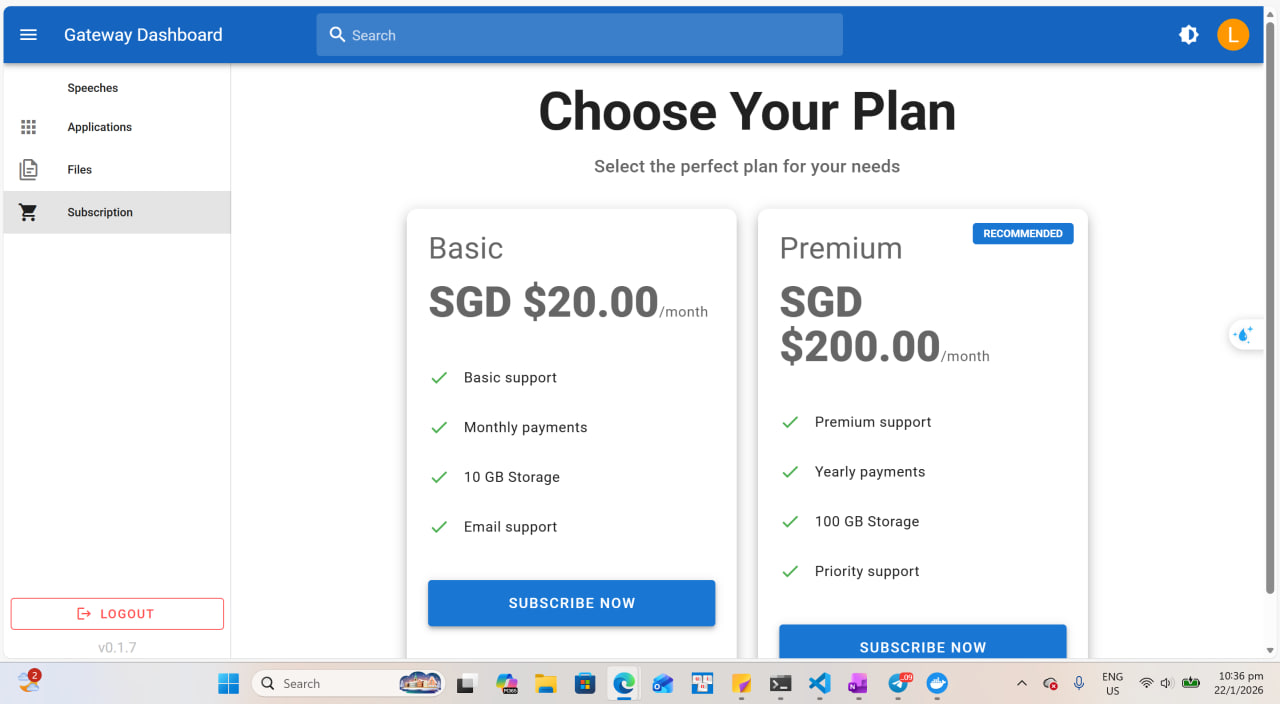
\includegraphics[width=0.8\textwidth]{images/Deployment/subscription-UI-for-users.jpg}
    \caption{Subscription Management Interface}
    \label{fig:subscription-ui}
\end{figure}

\begin{figure}[H]
    \centering
    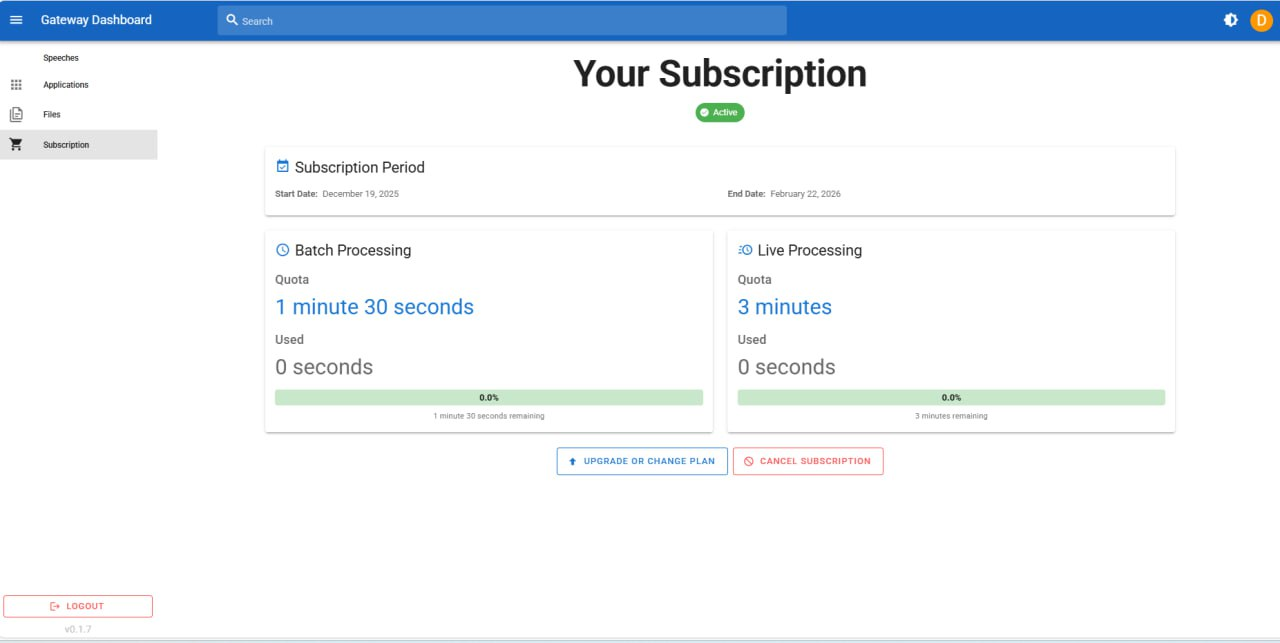
\includegraphics[width=0.8\textwidth]{images/Deployment/succesful-subscription.jpg}
    \caption{Successful Subscription Confirmation}
    \label{fig:successful-subscription}
\end{figure}

\subsection{Frontend Dashboard}

\textbf{Before:} No visual interface existed, requiring direct API calls for all operations and making it difficult to monitor subscriptions or manage users.

\textbf{After:} The dashboard provides a complete user experience. After authenticating via SSO or traditional login, users can view their subscription status and usage quotas, manage their profile, and upgrade or change plans. Administrators have access to additional tools for managing users, configuring subscription plans, and monitoring the overall system.

\begin{figure}[H]
    \centering
    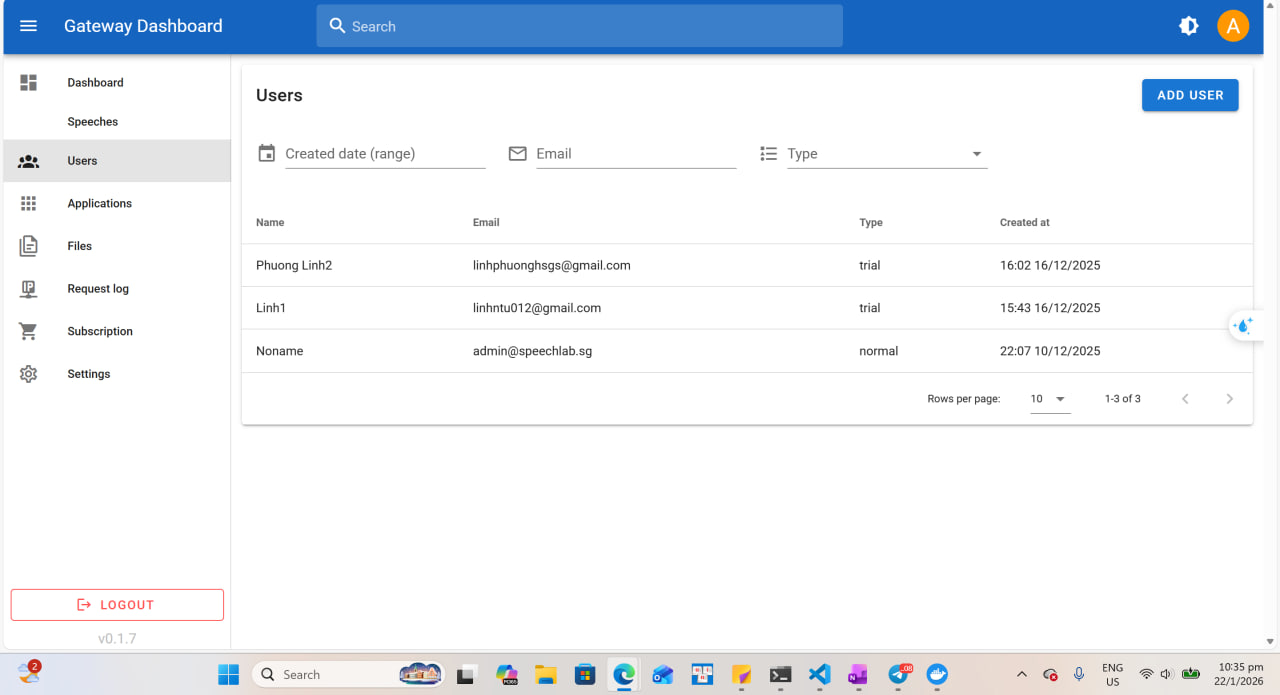
\includegraphics[width=0.8\textwidth]{images/Deployment/users-UI.jpg}
    \caption{User Management Dashboard}
    \label{fig:users-dashboard}
\end{figure}

\begin{figure}[H]
    \centering
    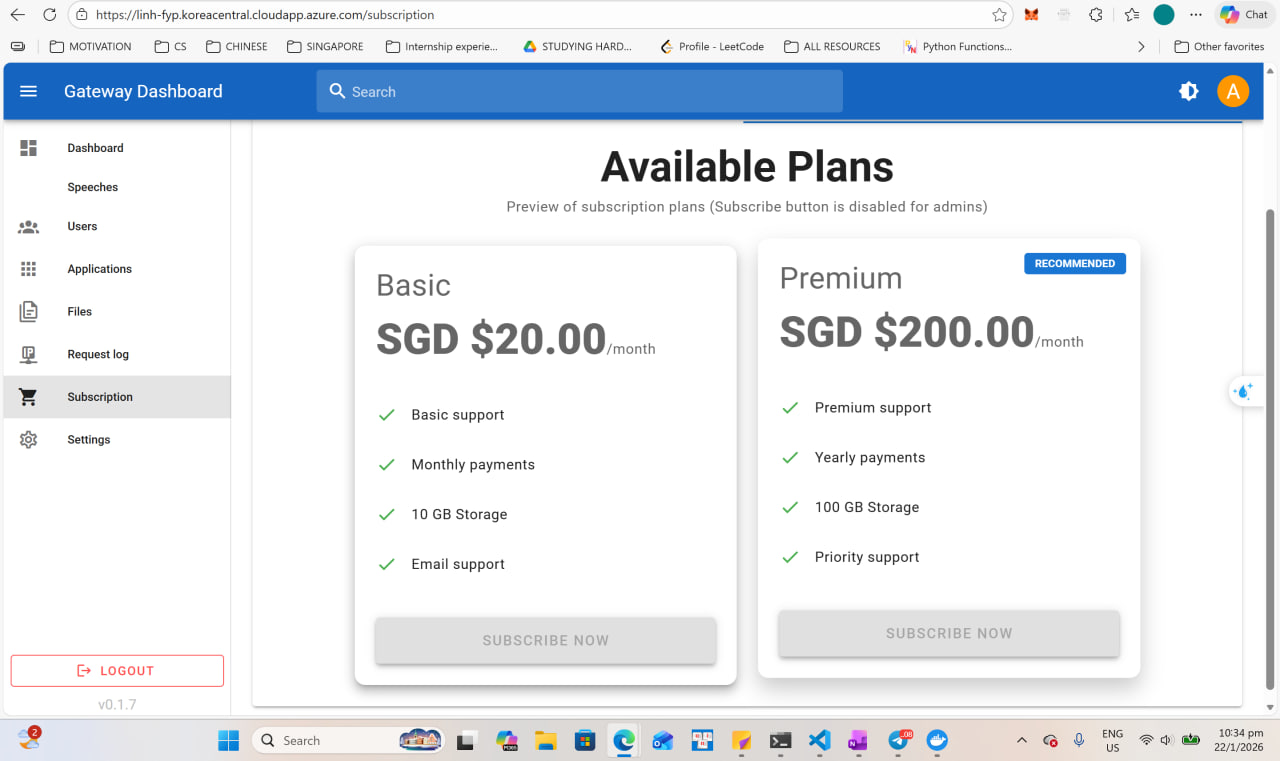
\includegraphics[width=0.8\textwidth]{images/Deployment/subscription-UI-for-admin.jpg}
    \caption{Admin Subscription Management Interface}
    \label{fig:admin-subscription}
\end{figure}

\begin{figure}[H]
    \centering
    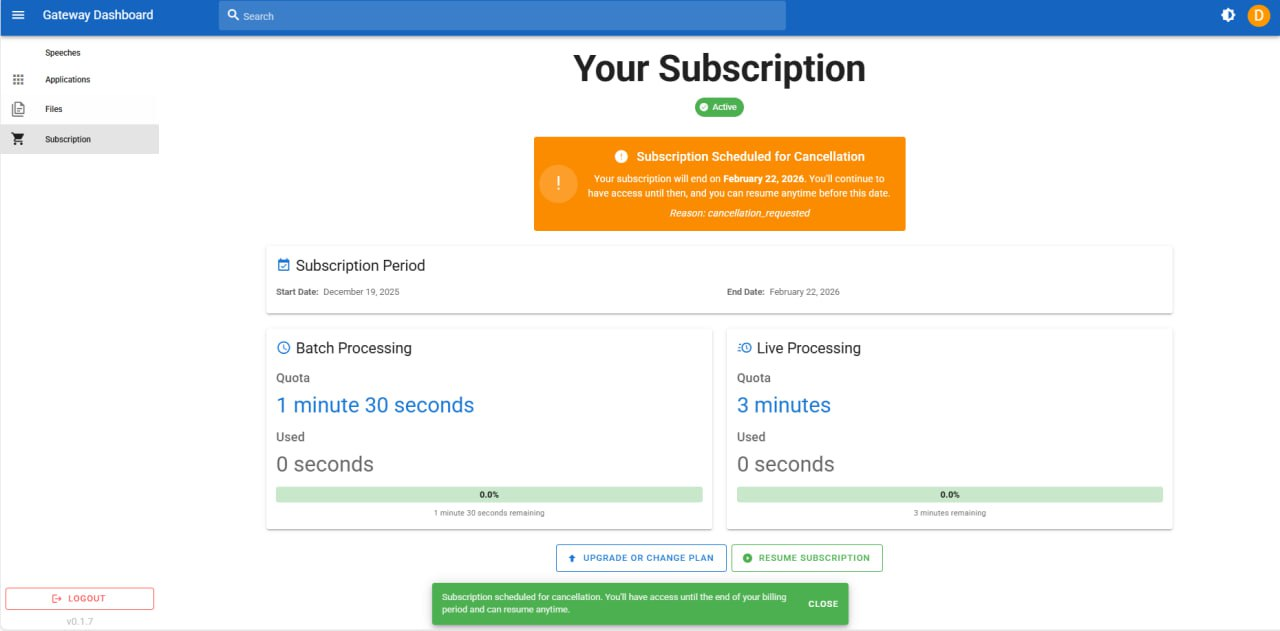
\includegraphics[width=0.8\textwidth]{images/Deployment/upgrade-or-change-plan.jpg}
    \caption{Plan Upgrade Interface}
    \label{fig:upgrade-plan}
\end{figure}
